\documentclass[12pt]{article}
% format
% \usepackage[a4paper, total={6in, 9in}]{geometry}                         

% math symbols
\usepackage{amsmath}
\usepackage{amsthm}
\usepackage{amssymb}
\usepackage[shortlabels]{enumitem} 
\usepackage{mathtools}
\usepackage{bbm}

% annotations
\setlength{\marginparwidth}{2cm}
\usepackage{soul}
\usepackage{pdfcomment}

% figures
\usepackage{graphicx}
\usepackage{subcaption}

% theorems
\theoremstyle{definition}
\newtheorem{thm}{Theorem}
\newtheorem{prop}[thm]{Proposition}
\newtheorem{lemma}[thm]{Lemma}
\newtheorem{rmk}[thm]{Remark}
\newtheorem{defn}[thm]{Definition}
\newtheorem{cor}[thm]{Corollary}
\newtheorem{exo}[thm]{Exercise}
\newtheorem{fact}[thm]{Fact}

% definition equal
\newcommand{\defeq}{\vcentcolon=}
\newcommand{\eqdef}{=\vcentcolon}
\pdfcommentsetup{color=yellow, opacity=0.5}

% bibliography
\usepackage[backend=biber,style=alphabetic, sorting=ynt]{biblatex}
\bibliography{ref}

% url highlight
\usepackage{hyperref}

% algos
\usepackage[linesnumbered,ruled,vlined]{algorithm2e}
\SetArgSty{textnormal}

% bullet point style
% \renewcommand{\labelitemi}{\tiny$\blacksquare$}

% new commands
\DeclareMathOperator{\dom}{dom}
\DeclareMathOperator{\Hess}{\textbf{H}}
\DeclareMathOperator{\Diag}{Diag}
\DeclareMathOperator{\Tr}{Tr}
\DeclareMathOperator{\ind}{i}
\DeclareMathOperator{\sgn}{sign}

% figures
\usepackage{tikz}
\usepackage{caption}

% colors
\definecolor{azure}{RGB}{41, 50, 65}
\definecolor{orange}{RGB}{238, 108, 77}
\definecolor{lightblue}{RGB}{224, 251, 252}
\definecolor{blue}{RGB}{152, 193, 217}
\definecolor{darkblue}{RGB}{61, 90, 128}
\definecolor{green}{RGB}{67, 170, 139}
\definecolor{purple}{RGB}{199, 125, 255}

% tikz setup
\def\rxhalf{0.5/2}
\def\ryhalf{0.4/2}

\def\rxone{1.0/2}
\def\ryone{0.7/2}

\def\rxonepoint{1.5/2}
\def\ryonepoint{0.9/2}

\def\rxtwo{2.0/2}
\def\rytwo{1.3/2}

\def\rxstwopoint{(3 - 1.5/2)/2}
\def\rxtwopoint{2.5/2}
\def\rytwopoint{1.5/2}

\def\rxthree{3/2}
\def\rythree{1.7/2}

\def\rxfour{4/2}
\def\ryfour{2/2}

\def\rxfourpoint{4.5/2}
\def\ryfourpoint{2.3/2}

\def\rxfive{5/2}
\def\ryfive{3.0/2}

\def\rxfivepoint{5.5/2}
\def\ryfivepoint{3.0/2}

\def\rxsix{6/2}
\def\rysix{3.3/2}

\begin{document}

    \section{Introduction and first definitions}

    We define polygon-circle
    graphs as the intersection
    graphs of polygons
    (including segments)
    inscribed in a circle.
    The aim of this text is to
    prove the following.

    \begin{thm} \label{thm:main}
        Triangle-free
        polygon-circle graphs
        have chromatic number at
        most 5.
    \end{thm}

    Without loss of generality,
    we will only consider
    families of polygons
    in which no two
    vertices coincide.

    We handle polygon-circle graphs by looking
    at the stereographic projection
    of the circle onto $\mathbb{R}$.
    Thus, a polygon-circle
    graph is represented by a 
    family $\left\{h_{i}\right\}_{i=1}^{n}$
    with 
    $h_{i} = \left(a_{1}^{\left(i\right)},
    \ldots, a_{k_{i}}^{\left(i\right)}\right)$ 
    for some $k_{i} \geq 2$ 
    with $a^{\left(i\right)}_{j} \in \mathbb{R}$
    being the image of
    the stereographic projection
    of a vertex of
    the corresponding 
    vertex of $h_{i}$.

    Given a familiy
    $F = \left\{h_{i}\right\}_{i=1}^{n}$ 
    of polygons, we denote
    the corresponding
    intersection graph $G\left(F\right)$
    and we say that
    $F$ is a polygon
    representation
    of $G\left(F\right)$.
    By abuse of notation,
    we will denote
    $\omega\left(G\left(F\right)\right)$ 
    by $\omega\left(F\right)$.
    Given two polygons
    $h_{i}, h_{i'}$ in $F$,
    we say that $h_{i}$ and
    $h_{i'}$ overlap 
    if there exists indices 
    $j$ and $j'$ such that
    $\left(a_{j}^{\left(i\right)},
     a_{j+1}^{\left(i\right)}\right)$ 
     and $\left(a_{j'}^{\left(i'\right)},
     a_{j'+1}^{\left(i'\right)}\right)$ 
     overlap.

     Given a polygon
     $h \defeq \left(
     a_{1}, \ldots, a_{k}\right)$,
     a contraction of $h$,
     is a polygon $h'$ 
     of the form
     $\left(a_{1}, \ldots,
     a_{i-1}, a_{i+1}, \ldots
     a_{k}\right)$ 
     where indices are
     unerstood modulo $k$.
     Consider a family of
     polygons
     $F = \left\{h_{i}\right\}_{i=1}^{n}$.
     Let $F'$ be the family
     of polygons generated
     by contracting one
     polygon in $F$.
     We define the partial order
     `$\prec$' on the set
     of polygon-circle graphs
     to be the smallest order
     containing
     the relations of the
     form $F' \prec F$.
     Notice that $\prec$ is
     well-founded since,
     when $F' \prec F$,
     the total number of 
     vertices of polygons in
     $F'$ is strictly less than
     that of the polygons in $F$.
     Thus, we cannot have an
     infinite decreasing sequence,
     $\cdots \prec F'' \prec F' \prec F$.

     Let $c \in \mathbb{R}$.
     We establish the following notation.
     \begin{align*}
         F^{0}\left(c\right) &\defeq
         \left\{h_{i} \in F \;\middle|\;
         a_{1}^{\left(i\right)}
         < c < a_{k_{i}}^{\left(i\right)}\right\}, \\
         F^{+}\left(c\right) &\defeq
         \left\{h_{i} \in F \;\middle|\;
         c < a_{1}^{\left(i\right)}\right\},\\
         F^{-}\left(c\right) &\defeq
         \left\{h_{i} \in F
         \;\middle|\; a_{k_{i}}^{\left(i\right)} < c\right\}.
     \end{align*}
     We also importantly define for
     $1 \leq i \leq n$ and 
     $1 < j \leq k_{i}$, 
     the following:
     \begin{gather*}
         \widetilde{F}^{0}\left(a_{j}^{\left(i\right)}\right)
         \defeq \left\{
         h_{i'} \in F \;\middle|\;
         a_{1}^{\left(i\right)} < a_{j'}^{\left(i'\right)}
         < a_{j}^{\left(i\right)}
         < a_{j'+1}^{\left(i'\right)}
         \text{ for some }
         1 \leq j' < k_{i'} \right\}.
     \end{gather*}
     For any $h_{i} \in F^{0}\left(c\right)$,
     denote $I_{c}\left(h_{i}\right)
     \defeq \left(a_{j}^{\left(i\right)},
     a_{j+1}^{\left(i\right)}\right)$ 
     such that $c \in 
     \left(a_{j}^{\left(i\right)},
     a_{j+1}^{\left(i\right)}\right)$ 
     and $O_{c}\left(h_{i}\right)
     \defeq \left(a_{1}^{\left(i\right)},
     a_{k_{i}}^{\left(i\right)}\right)$.
     For any polygon $h_{i}$,
     we call the segment
     $\left(a_{1}^{\left(i\right)},
     a_{k_{i}}^{\left(i\right)}\right)$
     the external
     segment of $h_{i}$.

     Also, let 
     $h_{i}$, $h_{i'}$ be two
     whose external segments
     overlap with
     $a_1^{\left(i\right)} < a_1^{\left(i'\right)}$.
     Let $\left(a_{j}^{\left(i\right)},
     a_{j+1}^{\left(i\right)}\right) =
     I_{a_1^{\left(i'\right)}}\left(h_{i}\right)$
     and let
     $b^{\left(i, i'\right)} \defeq a_{j+1}^{\left(i\right)}$.
     Let $\left(a_{j'}^{i'}, a_{j'+1}^{\left(i'\right)}\right)
     = I_{b^{\left(i,i'\right)}}\left(h_{i'}\right)$ 
     and let $a^{\left(i,i'\right)}
     \defeq a_{j'}^{\left(i'\right)}$.
     Similarly, let
     $\left(a^{\left(i'\right)}_{l'},
     a^{\left(i'\right)}_{l'+1}\right)
     = I_{a^{\left(i\right)}_{k_{i}}}\left(h_{i'}\right)$ 
     and let $c^{\left(i,i'\right)}
     \defeq a^{\left(i'\right)}_{l'}$.
     Let $\left(a^{\left(i\right)}
     _{l}, a^{\left(i\right)}_{l+1}\right)
     = I_{c^{\left(i, i'\right)}}\left(h_{i}\right)$
     and let 
     $d^{\left(i, i'\right)} \defeq
     a^{\left(i\right)}_{j+1}$.
     An illustration of 
     this is shown in Figure \ref{figure:overlap}.

     \begin{figure}[ht] 
     \begin{center}
     \resizebox{\textwidth}{!}{%
     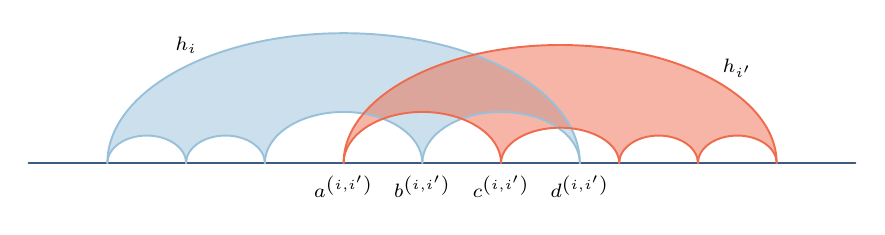
\begin{tikzpicture}[line width=0.7pt, line cap=round]

         \node[font=\scriptsize] at (1, 1.5)
         {$h_i$};
         \node[font=\scriptsize] at (8, 1.2)
         {$h_{i'}$};

         \node[font=\scriptsize] at (3,-0.3) {$a^{\left(i,i'\right)}$};
         \node[font=\scriptsize] at (4,-0.3) {$b^{\left(i,i'\right)}$};
         \node[font=\scriptsize] at (5,-0.3) {$c^{\left(i,i'\right)}$};
         \node[font=\scriptsize] at (6,-0.3) {$d^{\left(i,i'\right)}$}; 

         \path[fill=blue, opacity = 0.5]
             (0, 0)
             arc[start angle=180, end angle=0, x radius=\rxsix, y radius=\rysix] -- 
             (6, 0)
             arc[start angle=180, end angle=0, x radius=-\rxtwo, y radius=\rytwo] --
             (4, 0)
             arc[start angle=180, end angle=0, x radius=-\rxtwo, y radius=\rytwo] --
             (2, 0)
             arc[start angle=180, end angle=0, x radius=-\rxone, y radius=\ryone] --
             (1, 0)
             arc[start angle=180, end angle=0, x radius=-\rxone, y radius=\ryone] --
             cycle;

         \path[fill=orange, opacity=0.5]
             (3, 0) 
             arc[start angle=180, end angle=0, x radius=\rxfivepoint, y radius=\ryfivepoint] --
             (8.5, 0) 
             arc[start angle=180, end angle=0, x radius=-\rxone, y radius=\ryone] --
             (7.5, 0) 
             arc[start angle=180, end angle=0, x radius=-\rxone, y radius=\ryone] --
             (6.5, 0) 
             arc[start angle=180, end angle=0, x radius=-\rxonepoint, y radius=\ryonepoint] --
             (5, 0) 
             arc[start angle=180, end angle=0, x radius=-\rxtwo, y radius=\rytwo] --
             cycle;

         \draw[darkblue] (-1,0) -- (9.5, 0);

         \draw[blue] (0, 0) arc[start angle=180, end angle=0, x radius=\rxone, y radius=\ryone];
         \draw[blue] (1, 0) arc[start angle=180, end angle=0, x radius=\rxone, y radius=\ryone];
         \draw[blue] (2, 0) arc[start angle=180, end angle=0, x radius=\rxtwo, y radius=\rytwo];
         \draw[blue] (4, 0) arc[start angle=180, end angle=0, x radius=\rxtwo, y radius=\rytwo];
         \draw[blue] (0, 0) arc[start angle=180, end angle=0, x radius=\rxsix, y radius=\rysix];

         \draw[orange] (3, 0) arc[start angle=180, end angle=0, x radius=\rxtwo, y radius=\rytwo];
         \draw[orange] (5, 0) arc[start angle=180, end angle=0, x radius=\rxonepoint, y radius=\ryonepoint];
         \draw[orange] (6.5, 0) arc[start angle=180, end angle=0, x radius=\rxone, y radius=\ryone];
         \draw[orange] (7.5, 0) arc[start angle=180, end angle=0, x radius=\rxone, y radius=\ryone];
         \draw[orange] (3, 0) arc[start angle=180, end angle=0, x radius=\rxfivepoint, y radius=\ryfivepoint];

     \end{tikzpicture}
     }
     \end{center}
     \caption{}
     \label{figure:overlap}
     \end{figure} 

     \begin{rmk} \label{rmk:disj}
      By definition,
     $a^{\left(i, i'\right)} < b^{\left(i, i'\right)}$,
     $c^{\left(i, i'\right)} < d^{\left(i,i'\right)}$ 
     and $a^{\left(i, i'\right)} 
     \leq c^{\left(i, i'\right)}$,
     $b^{\left(i, i'\right)}
     \leq d^{\left(i, i'\right)}$.
     We thus either have, 
     $a^{\left(i, i'\right)} < 
     b^{\left(i, i'\right)} <
     c^{\left(i, i'\right)} < 
     d^{\left(i, i'\right)}$,
     in which case
     the intervals
     $\left(a^{\left(i, i'\right)},
     b^{\left(i,i'\right)}\right)$ 
     and
     $\left(c^{\left(i, i'\right)},
     d^{\left(i,i'\right)}\right)$
     are disjoint.
     Or we have
     $a^{\left(i,i'\right)} 
     \leq c^{\left(i, i'\right)}
     < b^{\left(i, i'\right)}
     \leq d^{\left(i, i'\right)}$.
     In this case, 
     since $c^{\left(i, i'\right)}$ 
     is a vertex of
     $h_{i'}$ and
     $c^{\left(i, i'\right)}
     < b^{\left(i, i'\right)}$, 
     we have that
     $a^{\left(i, i'\right)}
     \geq c^{\left(i,i'\right)}$ 
     and thus 
     $a^{\left(i, i'\right)}
     = c^{\left(i,i'\right)}$.
     By a similar
     reasoning, we get
     that $b^{\left(i,i'\right)}
     = d^{\left(i, i'\right)}$
     and so that
     $\left(a^{\left(i,i'\right)},
     b^{\left(i, i'\right)}\right) =
     \left(c^{\left(i,i'\right)},
     d^{\left(i, i'\right)}
     \right)$.
     \end{rmk}   

     Now, consider the set of intervals
     of the form $\left(a^{\left(i,i'\right)},
     b^{\left(i,i'\right)}\right)$ 
     or $\left(c^{\left(i, i'\right)},
     d^{\left(i, i'\right)}\right)$
     and denote it $P\left(F\right)$.
     Take the inclusion-wise maximal
     subfamily of such intervals
     and denote it $P^{0}\left(F\right)
     \subseteq P\left(F\right)$.
     
     \begin{rmk}
         Notice that, if 
         $\omega\left(F\right) = 2$,
         the maximality of
         $P^{0}\left(F\right)$,
         together with 
         Remark \ref{rmk:disj}
         implies that all the
         intervals in $P^{0}\left(F\right)$
         are disjoint.
     \end{rmk}

     From now on, consider
     $F = \left\{h_{i}\right\}_{i = 1}^{n}$ 
     be a family of polygons
     with $\omega\left(F\right)=2$.
     We remark the following
     two facts which we 
     state without proving them.

     \begin{fact} \label{fact:single}
         For any $a_{j}^{\left(i\right)}$,
         the elements of
         $\widetilde{F}^{0}\left(a_{j}^{\left(i\right)}\right)$ 
         are nested. That is, let
             $\widetilde{F}^{0}\left(a_{j}^{\left(i\right)}\right) 
             \eqdef \left\{h_1, \ldots, h_{l}\right\}$.
         Then, up to relabeling
         the elements of $F$, we have that
         \begin{gather*}
             I_{a_{j}^{\left(i\right)}}\left(h_1\right)
             \subseteq I_{a_{j}^{\left(i\right)}}\left(h_2\right)
             \subseteq \cdots
             \subseteq I_{a_{j}^{\left(i\right)}}\left(h_{l}\right), \\
             O_{a_{j}^{\left(i\right)}}\left(h_1\right)
             \subseteq O_{a_{j}^{\left(i\right)}}\left(h_2\right)
             \subseteq \cdots
             \subseteq O_{a_{j}^{\left(i\right)}}\left(h_{l}\right).
         \end{gather*}
     \end{fact}
     
     \begin{fact} \label{fact:double}
         For any two polygons
         $h \in \widetilde{F}^{0}\left(a_{j}^{\left(i\right)}\right)$ 
         and 
         $h' \in \widetilde{F}^{0}\left(a_{j'}^{\left(i\right)}\right)$, 
         we have that $h$ and $h'$
         do not overlap.    
     \end{fact}

     \section{Coloring plain polygon-circle graphs}

     We define a particular
     kind of circle graphs
     whose properies
     will be useful for the
     proof of Theorem \ref{thm:main}.

     \begin{defn} \label{def:plain}
         We call a polygon-circle graph plain,
         if it has a
         polygon representation
         $F \defeq \left\{h_{i}\right\}_{i = 1}^{n}$ 
         with $\omega\left(F\right) = 2$
         and such that, 
         for any 
         $\left(a, b\right) \in 
         P^{0}\left(F\right)$,
         there is no $h_{i}$ 
         such that
         $a < a_1^{\left(i\right)} < 
         a_{k_{i}}^{\left(i\right)} <
         b$.
     \end{defn}

     Plain polygon-circle graphs have the
     following property. 
     We note that we will
     be repeatedly using
     Fact \ref{fact:single}
     and Fact \ref{fact:double}
     without reference.

     \begin{lemma} \label{lemma:poly}
         Let $G$ be a plain polygon-circle graph and
         let $F \defeq \left\{h_{i}\right\}_{i =1}^{n}$ 
         be a polygon representation of $G$ with
         the properties
         required by Definition
         \ref{def:plain}
         Then $\chi\left(F\right) \leq 3$.
         Moreover, there exists
         a 3-coloring of $F$ such
         that for all $1 \leq i \leq n$
         and $1 < j \leq k_{i}$,
         all polygons in
         $\widetilde{F}^{0}\left(a_{j}^{\left(i\right)}\right)$
         have the same color.
         We call such coloring a
         `good coloring'.
     \end{lemma}

     \begin{proof}
         By way of contradiction,
         suppose that the statement is
         false and let
         $F = \left\{h_{i}\right\}_{i = 1}^{n}$ 
         be the smallest counterexample
         to this lemma with respect
         to the order $\prec$.
         Up to relabeling the elements
         of $F$, suppose without loss
         of generality that
         $h_{1}, \ldots, h_{t}$ are
         the polygons of $F$ whose
         external segments (seen as itervals
         of the form
         $\left(a_1^{\left(i\right)}, a_{k_{i}}^{\left(i\right)}\right)$) 
         are not contained
         in the external segment of 
         any other polygon of $F$.
         We further assume that
         $a_1^{\left(1\right)} <
         a_1^{\left(2\right)} < \ldots < 
         a_1^{\left(t\right)}$.
         By the minimality of $F$, we get
         that $G\left(F\right)$ is
         connected and $h_{i} \cap h_{i+1} \neq \emptyset$
         for all $i \in \left\{1, \ldots, t-1\right\}$.
         Therefore, we have that the points
         $a^{\left(i, i+1\right)}$ and
         $b^{\left(i, i+1\right)}$ are
         well-defined for all 
         $i \in \left\{1, \ldots, t-1\right\}$.
         
         \begin{itemize}
             \item First, suppose that $t = 1$.
             In this case, we have $F^{0}\left(a_1^{\left(1\right)}\right)
             = \emptyset$ and
             $F^{0}\left(a_{k_1}^{\left(1\right)}\right) = \emptyset$.
             Thus, contracting
             $a_{k_{i}}^{\left(1\right)}$ in $h_1$,
             either does not change the underlying graph,
             or implies that $G\left(F\right)$ is
             disconnected. In both cases, we have a contradiction.

             \item We are now going to prove that
             for all $i \in \left\{1, \ldots, t -1\right\}$,
             we have either $F^{-}\left(b^{\left(i, i+1\right)}\right)
             = \emptyset$ or 
             $F^{+}\left(a^{\left(i, i+1\right)}\right)
             = \emptyset$. This is
             not the case for $t \geq 4$ since,
             in such case, we would have 
             $h_1 \in F^{-}\left(b^{\left(2, 3\right)}\right)$
             and $h_{t} \in F^{+}\left(a^{\left(2, 3\right)}\right)$.
             Thus, this would imply $t \leq 3$.

             By way of contradiction,
             suppose that there exists
             $i_0 \in \left\{1, \ldots, t-1\right\}$
             such that $F^{-}\left(b^{\left(i_0, i_0+1\right)}\right)
             \neq \emptyset$ and
             $F^{+}\left(a^{\left(i_0, i_0+1\right)}\right)
             \neq \emptyset$.
             By the minimality of $F$, 
             we have that
             $F_1 \defeq F \setminus F^{+}
             \left(a^{\left(i_0, i_0+1\right)}\right)$
             and
             $F_2 \defeq F \setminus F^{-}
             \left(b^{i_0,i_0+1}\right)$ 
             admit good colorings
             $f_1$ and $f_2$.
             Notice that $F_1 \cap F_2 = 
             \left\{h_{i_0}, h_{i_0+1}\right\}$.
             So, we can assume without loss
             of generality that
             $f_1\left(h_{i_0}\right) = 
             f_2\left(h_{i_0}\right) = 1$ 
             and $f_1\left(h_{i_0+1}\right) =
             f_2\left(h_{i_0+1}\right) =2$.
             This also allows us to define 
             the function $f \vcentcolon 
             F \longrightarrow \left\{1, 2, 3\right\}$ 
             as follows:
             \begin{equation*}
                f\left(h\right) = 
                \begin{cases}
                    f_1\left(h\right) &\text{ if } h \in F_1, \\
                    f_2\left(h\right) &\text{ if } h \in F_{2}.
                \end{cases}
            \end{equation*} 
             By the maximality
             of $h_{i_0}$ and $h_{i_0+1}$,
             a family
             $\widetilde{F}^{0}\left(a_{j}^{\left(i\right)}\right)$
             is either entirely contained
             into $F_1$ or $F_2$.
             Thus, if $f$ is a coloring,
             it is also a good coloring.

             We now prove that $f$ is a coloring.
             Let $h_{i}, h_{i'} \in F$ be overlapping
             polygons. If both $h_{i}, h_{i'} \in F_1$ 
             or $h_{i}, h_{i'} \in F_2$, then 
             $f\left(h_{i}\right) \neq f\left(h_{i'}\right)$
             by the fact that $f_1$ and $f_2$ 
             are colorings.
             Suppose that $h_{i} \in F_1$ and
             $h_{i'} \in F_2$, then, since for no
             $\left(a, b\right) \in P^{0}\left(F\right)$ 
             and $h_{i} \in F$ we have
             $a < a_{1}^{\left(i\right)} <
             a_{k_{i}}^{\left(i\right)} < b$, we deduce that
             \begin{gather*}
                 a_1^{\left(i\right)} < 
                 a^{\left(i_0, i_0+1\right)} <
                 a_1^{\left(i'\right)} < 
                 a_{k_{i}}^{\left(i\right)} < 
                 b^{\left(i_0, i_0+1\right)} < 
                 a_{k_{i'}}^{\left(i'\right)}.
             \end{gather*}
             Now, since $h_{i_0+1}, h_{i'} \in 
             \widetilde{F}^{0}\left(b^{\left(i_0, i_0+1\right)}\right)$,
             and $h_{i_0+1}, h_{i'} \in F_2$,
             since $f_2$ is a good
             coloring, we have that $f\left(h_{i'}\right) =
             f\left(h_{i_0+1}\right) = 2$.
             Now, since $h_{i_0+1}$ and $h_{i}$ 
             overlap, 
             $h_{i_0+1}, h_{i} \in F_1$,
             and $f_1$ is a coloring, we get
             that $f\left(h_{i_0+1}\right) \neq
             f\left(h_{i}\right)$.
             Therefore, $f\left(h_{i}\right) \neq 
             f\left(h_{i'}\right) = 2$.
             So $f$ is a coloring and so,
             it is a good coloring.
             This contradicts the definition
             of $F$.

             We thus conclude that
             $F^{-}\left(b^{\left(i, i+1\right)}\right) = \emptyset$ 
             or $F^{+}\left(a^{\left(i, i+1\right)}\right) = \emptyset$
             for all $i \in \left\{1, \ldots, t-1\right\}$ and
             $t \leq 3$.

             \item Suppose now that $t = 2$.
             Suppose that there exists
             $b^{\left(1,2\right)} < 
             a_{j}^{\left(2\right)} <
             a_{k_2}^{\left(2\right)}$.
             Then, since $F^{0}\left(a_{k_2}^{\left(2\right)}\right) = 
             \emptyset$, we have that 
             contracting $a_{k_2}^{\left(2\right)}$
             in $h_2$, does not change the underlying 
             graph. Which is not possible by
             the definition of $F$.
             therefore $a^{\left(1,2\right)} =
             a_{k_2-1}^{\left(2\right)}$. By a
             symmetric reasoning, we can show
             $b^{\left(1, 2\right)} = a_2^{\left(1\right)}$.
             We have the setting shown in Figure \ref{figure:t=2}.

             \begin{figure}[ht]
             \begin{center}
             \resizebox{\textwidth}{!}{%
             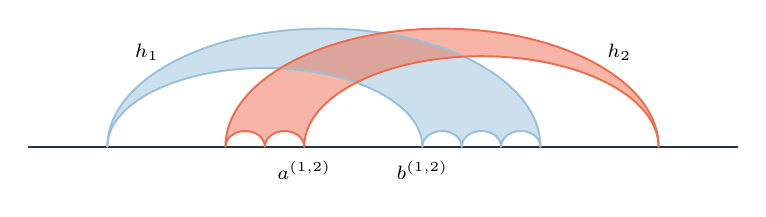
\begin{tikzpicture}[line width=0.7pt, line cap=round]

                 \node[font=\scriptsize] at (0.5, 1.2) {$h_1$};
                 \node[font=\scriptsize] at (6.5, 1.2) {$h_2$};
 
                 \node[font=\scriptsize] at (2.5, -0.3) {$a^{\left(1, 2\right)}$};
                 \node[font=\scriptsize] at (4, -0.3) {$b^{\left(1, 2\right)}$};
 
                 \path[fill=blue, opacity=0.5] (0, 0)
                 arc[start angle=180, end angle=0, x radius=\rxfivepoint, y radius=\ryfivepoint] --
                 (5.5, 0)
                 arc[start angle=180, end angle=0, x radius=-\rxhalf, y radius=\ryhalf] --
                 (5, 0)
                 arc[start angle=180, end angle=0, x radius=-\rxhalf, y radius=\ryhalf] --
                 (4.5, 0)
                 arc[start angle=180, end angle=0, x radius=-\rxhalf, y radius=\ryhalf] --
                 (4, 0)
                 arc[start angle=180, end angle=0, x radius=-\rxfour, y radius=\ryfour];

                 \path[fill=orange, opacity=0.5]
                 (1.5, 0)
                 arc[start angle=180, end angle=0, x radius=\rxfivepoint, y radius=\ryfivepoint] --
                 (7, 0)
                 arc[start angle=180, end angle=0, x radius=-\rxfourpoint, y radius=\ryfourpoint] --
                 (2.5, 0)
                 arc[start angle=180, end angle=0, x radius=-\rxhalf, y radius=\ryhalf] --
                 (2, 0)
                 arc[start angle=180, end angle=0, x radius=-\rxhalf, y radius=\ryhalf];

                 \draw[azure] (-1,0) -- (8, 0);
 
                 \draw[blue] (0, 0)
                 arc[start angle=180, end angle=0, x radius=\rxfivepoint, y radius=\ryfivepoint];
                 \draw[blue] (5.5, 0)
                 arc[start angle=180, end angle=0, x radius=-\rxhalf, y radius=\ryhalf];
                 \draw[blue] (5, 0)
                 arc[start angle=180, end angle=0, x radius=-\rxhalf, y radius=\ryhalf];
                 \draw[blue] (4.5, 0)
                 arc[start angle=180, end angle=0, x radius=-\rxhalf, y radius=\ryhalf];
                 \draw[blue] (4, 0)
                 arc[start angle=180, end angle=0, x radius=-\rxfour, y radius=\ryfour];

                 \draw[orange] (1.5, 0)
                 arc[start angle=180, end angle=0, x radius=\rxfivepoint, y radius=\ryfivepoint];
                 \draw[orange] (7, 0)
                 arc[start angle=180, end angle=0, x radius=-\rxfourpoint, y radius=\ryfourpoint];
                 \draw[orange] (2.5, 0)
                 arc[start angle=180, end angle=0, x radius=-\rxhalf, y radius=\ryhalf];
                 \draw[orange] (2, 0)
                 arc[start angle=180, end angle=0, x radius=-\rxhalf, y radius=\ryhalf];

             \end{tikzpicture}
             }
             \end{center}
             \caption{}
             \label{figure:t=2}
             \end{figure}
             
             Consider the case of
             $F^{+}\left(a^{\left(1, 2\right)}\right) = \emptyset$.
             Since $b^{\left(1, 2\right)} =
             a_{2}^{\left(2\right)}$, $h_1$ only
             overlaps with $h_2$.
             By the minimality of $F$, 
             we get a good coloring 
             $f'$ of $F \setminus \left\{h_1\right\}$.
             We can extend $f'$ into 
             a good coloring of $F$,
             by coloring $h_1$ with 
             a color different from
             $f'\left(h_2\right)$.

             Consider the case of
             $F^{-}\left(b^{\left(1, 2\right)}\right) = \emptyset$.
             Since $a^{\left(1, 2\right)} = 
             a_{k_2}^{\left(2\right)}$,
             $h_2$ only overlaps with $h_1$.
             Now, take the outermost polygons
             overlapping with $h_1$:
             \begin{gather*}
                 \left\{u_{j}\right\}_{j = 1}^{s} = 
                 \left\{\left(c_1^{\left(j\right)}, \ldots,
                 c_{l_{j}}^{\left(j\right)}\right)\right\}_{j = 1}^{\left(s\right)}
             \end{gather*}
             with
             \begin{gather*}
                 c_1^{\left(1\right)} <
                 c_{l_1}^{\left(1\right)} <
                 c_1^{\left(2\right)} < 
                 \cdots <
                 c_{l_{s-1}}^{\left(s- 1\right)} <
                 c_1^{\left(s\right)} <
                 c_{l_{s}}^{\left(s\right)}.
             \end{gather*}

             This setting is illustrated in
             Figure \ref{figure:multi}.
             
             \begin{figure}[ht]
             \begin{center}
             \resizebox{\textwidth}{!}{%
             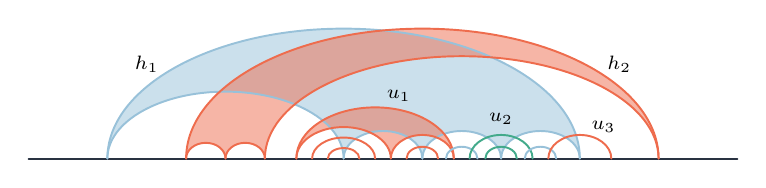
\begin{tikzpicture}[line width=0.7pt, line cap=round]
 
                 \path[fill=blue, opacity=0.5] (0, 0)
                 arc[start angle=180, end angle=0, x radius=\rxsix, y radius=\rysix] --
                 (6, 0)
                 arc[start angle=180, end angle=0, x radius=-\rxone, y radius=\ryone] --
                 (5, 0)
                 arc[start angle=180, end angle=0, x radius=-\rxone, y radius=\ryone] --
                 (4, 0)
                 arc[start angle=180, end angle=0, x radius=-\rxone, y radius=\ryone] --
                 (3, 0)
                 arc[start angle=180, end angle=0, x radius=-\rxthree, y radius=\rythree];
 
                 \path[fill=orange, opacity=0.5] (2.4, 0)
                 arc[start angle=180, end angle=0, x radius=\rxtwo, y radius=\rytwo] --
                 (4.4, 0)
                 arc[start angle=180, end angle=0, x radius=-0.8/2, y radius=0.6/2] --
                 (3.6, 0)
                 arc[start angle=180, end angle=0, x radius=-1.2/2, y radius=0.8/2];
 
                 \path[fill=orange, opacity=0.5] (1, 0)
                 arc[start angle=180, end angle=0, x radius=\rxsix, y radius=\rysix] --
                 (7, 0)
                 arc[start angle=180, end angle=0, x radius=-\rxfive, y radius=2.6/2] --
                 (2, 0)
                 arc[start angle=180, end angle=0, x radius=-\rxhalf, y radius=\ryhalf] --
                 (1.5, 0)
                 arc[start angle=180, end angle=0, x radius=-\rxhalf, y radius=\ryhalf];
 
                 \draw[azure] (-1, 0) -- (8, 0);
 
                 \draw[blue] (0, 0)
                 arc[start angle=180, end angle=0, x radius=\rxsix, y radius=\rysix];
                 \draw[blue] (6, 0)
                 arc[start angle=180, end angle=0, x radius=-\rxone, y radius=\ryone];
                 \draw[blue] (5, 0)
                 arc[start angle=180, end angle=0, x radius=-\rxone, y radius=\ryone];
                 \draw[blue] (4, 0)
                 arc[start angle=180, end angle=0, x radius=-\rxone, y radius=\ryone];
                 \draw[blue] (3, 0)
                 arc[start angle=180, end angle=0, x radius=-\rxthree, y radius=\rythree];
 
                 \draw[orange] (2.4, 0)
                 arc[start angle=180, end angle=0, x radius=\rxtwo, y radius=\rytwo];
                 \draw[orange] (4.4, 0)
                 arc[start angle=180, end angle=0, x radius=-0.8/2, y radius=0.6/2];
                 \draw[orange] (3.6, 0)
                 arc[start angle=180, end angle=0, x radius=-1.2/2, y radius=0.8/2];
 
                 \draw[orange] (2.6, 0)
                 arc[start angle=180, end angle=0, x radius=0.8/2, y radius=0.8/3];
 
                 \draw[orange] (2.8, 0)
                 arc[start angle=180, end angle=0, x radius=0.4/2, y radius=0.4/3];
 
                 \draw[orange] (3.8, 0)
                 arc[start angle=180, end angle=0, x radius=0.4/2, y radius=0.3/2];
                    
                 \draw[blue] (4.3, 0)
                 arc[start angle=180, end angle=0, x radius=0.4/2, y radius=0.3/2];

                 \draw[green] (4.6, 0)
                 arc[start angle=180, end angle=0, x radius=0.8/2, y radius=0.6/2];
 
                 \draw[green] (4.8, 0)
                 arc[start angle=180, end angle=0, x radius=0.4/2, y radius=0.3/2];
                
                 \draw[blue] (5.3, 0)
                 arc[start angle=180, end angle=0, x radius=0.4/2, y radius=0.3/2];

                 \draw[orange] (5.6, 0)
                 arc[start angle=180, end angle=0, x radius=0.8/2, y radius=0.6/2];
 
                 \draw[orange] (1, 0)
                 arc[start angle=180, end angle=0, x radius=\rxsix, y radius=\rysix];
                 \draw[orange] (7, 0)
                 arc[start angle=180, end angle=0, x radius=-\rxfive, y radius=2.6/2];
                 \draw[orange] (2, 0)
                 arc[start angle=180, end angle=0, x radius=-\rxhalf, y radius=\ryhalf];
                 \draw[orange] (1.5, 0)
                 arc[start angle=180, end angle=0, x radius=-\rxhalf, y radius=\ryhalf];
 
                 \node[font=\scriptsize] at (0.5, 1.2) {$h_1$};
                 \node[font=\scriptsize] at (6.5, 1.2) {$h_2$};
                 \node[font=\scriptsize] at (3.7, 0.8) {$u_1$};
                 \node[font=\scriptsize] at (5, 0.5) {$u_2$};
                 \node[font=\scriptsize] at (6.3, 0.4) {$u_3$};
                 
             \end{tikzpicture}
             }
             \end{center}
             \caption{}
             \label{figure:multi}
             \end{figure} 

             We can thus partition all the
             polygons overlapping with
             $h_1$ by looking at which $u_{j}$ 
             the are nested in. For any
             $1 \leq j \leq s$, denote
             by $N\left(u_{j}\right)$
             the class of polygons 
             nested in $u_{j}$.
             Notice that we have a good coloring
             $f'$ of $F \setminus \left\{h_2\right\}$.
             We can extend $f'$ into a colring
             $f$ of $F$ by coloring $h_2$ with
             the same color as the other polygons in
             $F^{0}\left(a_2^{\left(1\right)}\right)$.

             For the sake of simplicity,
             suppose that we have
             $f\left(h_1\right) = 1$,
             $f\left(u_1\right) = 2$ and
             $f\left(h_2\right) = 2$.
             Notice that all the polygons
             in a given class $N\left(u_{j}\right)$ 
             have the same color.

             In order to obtain a good coloring
             of $F$, it suffices to color all the polygons
             overlapping with $h_1$ with color 2.
             If one exists, take the smallest index
             $m$ ($\neq 1$) such that 
             the color of $N\left(u_{m}\right)$ 
             is different from 2. So $f\left(u_{m}\right) = 3$.
             Define $O \defeq F^{+}\left(c_{l_{m-1}}^{\left(m-1\right)}\right)$.
             Notice that the polygons 
             in $F \setminus O$, that overlap
             with polygons in $O$ lie in
             $F^{0}\left(c_{l_{m-1}}^{\left(m-1\right)}\right) =
             \widetilde{F}^{0}\left(c_{l_{m-1}}^{\left(m -1\right)}\right)$
             by the maximality of $u_{m-1}$.
             All polygons in
             $\widetilde{F}^{0}\left(c_{l_{m-1}}^{\left(m -1\right)}\right)$
             are colored
             with color 1.
             We can thus swap the colors
             2 and 3 of the polygons 
             contained in $O'$, so that
             the classes $N\left(u_1\right),
             \ldots, N\left(h_{l_{m}}\right)$ are
             colored with color 2.
             We can repeat this procedure until
             all classes $N\left(u_{j}\right)$ 
             are colored with color 2.
             
             We thus get a good coloring
             of $F$, which is a contradiction.

             \item We now tackle the case of $t = 3$.
             If $t = 3$, we have $h_3 \in F^{+}
             \left(a^{\left(1, 2\right)}\right)$ 
             and $h_1 \in F^{-}\left(b^{\left(2, 3\right)}\right)$.
             Thus, we have that $F^{+}\left(b^{\left(1, 2\right)}\right)
             \neq \emptyset$.
             By similar arguments as those
             used in the previous case,
             the minimality of $F$ implies
             $a^{\left(1, 2\right)} = a_1^{\left(2\right)}$,
             $b^{\left(1, 2\right)} = a_2^{\left(1\right)}$,
             $a^{\left(2, 3\right)} = a_{k_3 - 1}^{\left(3\right)}$ and
             $b^{\left(2, 3\right)} = a_{k_2}^{\left(2\right)}$.

             Also, suppose that there exists
             $a_2^{\left(1\right)} < a_{j}^{\left(2\right)} <
             a_{k_1}^{\left(1\right)}$ for
             some $j > 1$. Then,
             since $F^{-}\left(b^{\left(1, 2\right)}\right) = \emptyset$, 
             contracting $a_1^{\left(2\right)}$ 
             in $h_2$ does not change the
             underlying graph, which
             contradicts the definition of $F$.
             Similarly, there is no
             $j < k_2$ with $a_1^{\left(3\right)} <
             a_{j}^{\left(2\right)} <
             a_{k_3-1}^{\left(3\right)}$.
             Therefore, for all
             $1 < j < k_2$, we have
             that $a_{k_1}^{\left(1\right)} < 
             a_{j}^{\left(2\right)} < 
             a_1^{\left(3\right)}$.

             Suppose that there exists
             $1 < j < k$ such that
             $a_{k_1}^{\left(1\right)} <
             a_{j}^{\left(2\right)} <
             a_1^{\left(3\right)}$.
             The setting is illustrated
             in Figure \ref{figure:t=3}.
             
             \begin{figure}[ht]
             \begin{center}
             \resizebox{\textwidth}{!}{%
             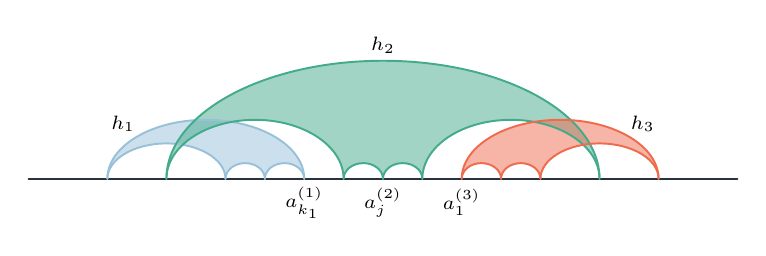
\begin{tikzpicture}[line width=0.7pt, line cap=round]
 
                 \node[font=\scriptsize] at (2.5, -0.3) {$a^{\left(1\right)}_{k_1}$};
                 \node[font=\scriptsize] at
                 (3.5, -0.3) {$a^{\left(2\right)}_j$};
                 \node[font=\scriptsize] at
                 (4.5, -0.3) {$a^{\left(3\right)}_1$};
 
                 \node[font=\scriptsize] at (0.2, 0.7) {$h_1$};
                 \node[font=\scriptsize] at (3.5, 1.7) {$h_2$};
                 \node[font=\scriptsize] at (6.8, 0.7) {$h_3$};
 
                 \path[fill=blue, opacity=0.5] (0, 0)
                 arc[start angle=180, end angle=0, x radius=\rxtwopoint, y radius=\rytwopoint]
                 -- (2.5, 0)
                 arc[start angle=180, end angle=0, x radius=-\rxhalf, y radius=\ryhalf]
                 -- (2, 0)
                 arc[start angle=180, end angle=0, x radius=-\rxhalf, y radius=\ryhalf]
                 -- (1.5, 0)
                 arc[start angle=180, end angle=0, x radius=-\rxonepoint, y radius=\ryonepoint];
 
                 \path[fill=green, opacity=0.5] (1.5/2, 0)
                 arc[start angle=180, end angle=0, x radius=\rxfivepoint, y radius=\ryfivepoint] --
                 (5.5 + 1.5/2, 0)
                 arc[start angle=180, end angle=0, x radius=-\rxstwopoint, y radius=\rytwopoint] --
                 (4, 0)
                 arc[start angle=180, end angle=0, x radius=-\rxhalf, y radius=\ryhalf] --
                 (3.5, 0)
                 arc[start angle=180, end angle=0, x radius=-\rxhalf, y radius=\ryhalf] --
                 (3, 0)
                 arc[start angle=180, end angle=0, x radius=-\rxstwopoint, y radius=\rytwopoint];
 
                 \path[fill=orange, opacity=0.5] (4.5, 0)
                 arc[start angle=180, end angle=0, x radius=\rxtwopoint, y radius=\rytwopoint] --
                 (7, 0)
                 arc[start angle=180, end angle=0, x radius=-\rxonepoint, y radius=\ryonepoint] --
                 (5.5, 0)
                 arc[start angle=180, end angle=0, x radius=-\rxhalf, y radius=\ryhalf] --
                 (5, 0)
                 arc[start angle=180, end angle=0, x radius=-\rxhalf, y radius=\ryhalf];
 
                 \draw[azure] (-1, 0) -- (8, 0);
 
                 \draw[blue] (0, 0)
                 arc[start angle=180, end angle=0, x radius=\rxtwopoint, y radius=\rytwopoint];
                 \draw[blue] (2.5, 0)
                 arc[start angle=180, end angle=0, x radius=-\rxhalf, y radius=\ryhalf];
                 \draw[blue] (2, 0)
                 arc[start angle=180, end angle=0, x radius=-\rxhalf, y radius=\ryhalf];
                 \draw[blue] (1.5, 0)
                 arc[start angle=180, end angle=0, x radius=-\rxonepoint, y radius=\ryonepoint];
 
                 \draw[green] (1.5/2, 0)
                 arc[start angle=180, end angle=0, x radius=\rxfivepoint, y radius=\ryfivepoint];
                 \draw[green] (5.5 + 1.5/2, 0)
                 arc[start angle=180, end angle=0, x radius=-\rxstwopoint, y radius=\rytwopoint];
                 \draw[green] (4, 0)
                 arc[start angle=180, end angle=0, x radius=-\rxhalf, y radius=\ryhalf];
                 \draw[green] (3.5, 0)
                 arc[start angle=180, end angle=0, x radius=-\rxhalf, y radius=\ryhalf];
                 \draw[green] (3, 0)
                 arc[start angle=180, end angle=0, x radius=-\rxstwopoint, y radius=\rytwopoint];
 
                 \draw[orange] (4.5, 0)
                 arc[start angle=180, end angle=0, x radius=\rxtwopoint, y radius=\rytwopoint];
                 \draw[orange] (7, 0)
                 arc[start angle=180, end angle=0, x radius=-\rxonepoint, y radius=\ryonepoint];
                 \draw[orange] (5.5, 0)
                 arc[start angle=180, end angle=0, x radius=-\rxhalf, y radius=\ryhalf];
                 \draw[orange] (5, 0)
                 arc[start angle=180, end angle=0, x radius=-\rxhalf, y radius=\ryhalf];
                 
             \end{tikzpicture}
             }
             \end{center}
             \caption{}
             \label{figure:t=3}
             \end{figure}

             Contract $a_{k_2}^{\left(2\right)}$ 
             in $h_2$ (call the resulting
             polygon $h_2'$)
             and get a good coloring
             $f'$ of the resulting family
             of polygons.
             Suppose without loss of
             generality that $f\left(h_1\right) = 1$,
             $f'\left(h_2'\right) = 2$.
             If $f'\left(h_3\right) \neq 2$, 
             then we can decontract $h_2'$ 
             to get a good coloring of $F$, 
             which is a contradiction.
             Let us consider the case
             $f'\left(h_3\right) = 2$.
             Define $O' \defeq F^{+}\left(a_{k_2 - 1}^{\left(2\right)}\right)$.
             Notice that all the polygons in
             $F \setminus O'$ that overlap with
             $O'$ lie in the set 
             $F^{0}\left(a_{k_2-1}^{\left(2\right)}\right) =
             \widetilde{F}^{0}\left(a_{k_2-1}^{\left(2\right)}\right)$
             by the maximality of $h_2$.
             By the fact that $f'$ is a
             good coloring, all polygons in $F^{0}\left(
             a_{k_2-1}^{\left(2\right)}\right)$
             share the same color $\gamma \in \left\{1, 3\right\}$.
             Let $\delta \in \left\{1, 3\right\} 
             \setminus \left\{\gamma\right\}$
             We can swap the colors 2 and $\delta$
             in $O'$ by preserving the good coloring 
             property.
             We can finally decontract $h_2$ to get
             a good coloring of $F$. 
             A contradiction.

             Thus, we deduce that $h_2$ is a segment.
             We get a good coloring $f'$ of
             $F \setminus \left\{h_2\right\}$.
             Suppose without loss of generality
             that $f'\left(h_1\right) = 1$.
             We define $u_1, \ldots, u_{s}$ 
             analogously as in the previous case.
             By the same argument as in the previous case,
             we can color all the sets 
             $N\left(u_{j}\right)$ with the
             same color as $N\left(u_1\right)$,
             say 2 without loss of generality.
             If after this recoloring,
             $f'\left(h_3\right) \neq 2$, 
             we can extend $f'$ into a
             good coloring of $F$ by 
             coloring $h_2$ with color 2.
             This gives a contradiction.
             
             We thus have $f'\left(h_3\right) = 2$.
             Let $\gamma \in \left\{1, 3\right\}$
             be the color of the polygons
             in $F^{0}\left(c_{l_{s}}^{\left(s\right)}\right)
             = \widetilde{F}^{0}\left(
             c_{l_{s}}^{\left(s\right)}\right)$.
             Let $O'' \defeq F^{+}\left(
             c_{l_{s}}^{\left(s\right)}\right)$.
             Notice that all the elements
             in $F \setminus O''$ 
             that overlap elements in $O''$
             are contained in $\widetilde{F}^{0}\left(
             c_{l_{s}}^{\left(s\right)}\right)$,
             and so have color $\gamma$.
             Let $\delta \in \left\{1, 3\right\}
             \setminus \left\{\gamma\right\}$.
             By the above discussion, we can swap colors
             2 and $\delta$ in $O''$
             by preserving the good coloring property.
             We can thus extend $f'$ into a
             good coloring of $F$ by
             coloring $h_2$ with color 2
             to obtain a good coloring of $F$.
             Again, a contradiction.
         \end{itemize} 
     We have the desired result. 
     \end{proof}

     \section{Proof of Theorem \ref{thm:main}}

     We first establish some more notation.
     Namely, using the same notational conventions
     used up to this point, we denote, for
     $1 \leq i' \leq n$ and $1 \leq j' < k_{i'}$
     \begin{gather*}
         \overline{F}^{0}\left(a_{j'}^{\left(i'\right)}\right) \defeq
         \left\{h_{i} \in F \;\middle|\;
         a_{j}^{\left(i\right)} <
         a_{j'}^{\left(i'\right)} <
         a_{j+1}^{\left(i\right)} <
         a_{k_{i'}}^{\left(i'\right)}
         \text{ for some }
         1 \leq j < k_{i}\right\}
     \end{gather*}
     
     We remark in passing that, by symmetry,
     Lemma \ref{lemma:poly} remains 
     true if we
     replace $\widetilde{F}^{0}\left(a_{j}^{\left(i\right)}\right)$ 
     with $\overline{F}^{0}\left(a_{j'}^{\left(i'\right)}\right)$,
     since this would be a mirrored version
     of such lemma.
      
     We now present our main result
     with similar techniques as the one
     employed in \cite{rus}.
     Again, in what follows, 
     we will repeatedly use
     Fact \ref{fact:single}
     and Fact \ref{fact:double}
     without reference.

     In particular, we prove the
     following  
     statement which clearly
     implies Theorem \ref{thm:main}.

     \begin{lemma}
         Let $F \defeq \left\{h_{i}\right\}_{i = 1}^{n}$ 
         with $\omega\left(F\right) = 2$.
         There exist (possibly overlapping)
         subfamilies
         $F_1, \ldots, F_{l}$ 
         of $F$ with $F = \cup_{i = 1}^{l} F_{i}$
         and precolorings
         $f_1, \ldots, f_{l}$ with
         $f_{k} \vcentcolon F'_{k} \defeq
         \cup_{i=1}^{k} F_{i} \longrightarrow
         \left\{1, 2, 3, 4, 5\right\}$
         for all $1 \leq k \leq l$
         such that the following holds
         for all $1 \leq k \leq l$.
         \begin{enumerate}
             \item \label{cond:1} The polygons
                 in $F \setminus F'_{k}$
                 do not overlap with 
                 intervals in 
                 $F'_{k-1} \setminus F_{k}$.
             \item \label{cond:2} The polygons
                 $h_{i} \in F \setminus  F'_{k}$ 
                 are such that 
                 $a < a_1^{\left(i\right)} <
                 a_{k_{i}}^{\left(i\right)} < b$
                 for some $\left(a, b\right)
                 \in P^{0}\left(F_{k}\right)$.
             \item \label{cond:3} For each
                 $p \defeq \left(a, b\right)
                 \in P^{0}\left(F_{k}\right)$,
                 either one color is used to
                 color all polygons in
                 $\overline{F}^{0}\left(k\right)
                 \left(a\right)$ and
                 no more than two colors
                 are used to color the polygons
                 in $\widetilde{F}^{0}_{k}\left(b\right)$
                 or viceversa,
                 only one color is used
                 to color the polygons
                 in $\widetilde{F}^{0}_{k}\left(b\right)$
                 and no more than
                 two colors are used to
                 color the polygons
                 in $\overline{F}^{0}_{k}\left(a\right)$. 
         \end{enumerate}
     \end{lemma}

     \begin{proof}
         Let $F = \left\{h_{i}\right\}_{i = 1}^{n}$
         be a family of polygons with
         $\omega\left(F\right) = 2$.
         We construct the subfamilies
         $F_1, \ldots, F_{k}, \ldots, F_{l}$ 
         and the precolorings
         $f_1, \ldots, f_{k}, \ldots, f_{l}$ 
         by induction on $k$.

         \begin{itemize}
             \item \textbf{Base case}.
                 Let $F_1 \subseteq F$
                 be the subset of polygons
                 $h_{i} \in F$ such that 
                 there is no $\left(a, b\right)
                 \in P^{0}\left(F\right)$
                 with $a < a_1^{\left(i\right)} <
                 a_{k_{i}}^{\left(i\right)} < b$.
                 By Lemma \ref{lemma:poly} there
                 exists a coloring of $F_1$
                 with colors $\left\{1, 2, 3\right\}$ 
                 such that for every $h_{i} \in F_1$ 
                 and $1 < j \leq k_{i}$,
                 the polygons in 
                 $\widetilde{F}^{0}\left(a_{j}^{\left(i\right)}\right)$ 
                 have the same color.
                 Let $f_1$ be such coloring.
                 Condition \ref{cond:1} trivially holds.
                 Condition \ref{cond:2} follows 
                 directly from the choice of $F_1$.
                 Condition \ref{cond:3} follows
                 from the choice of $f_1$ by
                 Lemma \ref{lemma:poly}.
             \item \textbf{Induction step}.
                 Consider that for some
                 $k \geq 1$, the families
                 $F_1, \ldots, F_{k}$
                 and the precolorings $f_1, \ldots, f_{k}$ 
                 have been constructed.
                 If $F \setminus F'_{k} = \emptyset$,
                 then $k = l$ and the
                 result follows.
                 Otherwise, we construct
                 $F_{k+1}$ and $f_{k+1}$ 
                 with the desired properties.

                 Consider any interval
                 $p = \left(a^{\left(i, i'\right)},
                 b^{\left(i, i'\right)}\right)
                 \in P^{0}\left(F_{k}\right)$,
                 such that there
                 exists $h_{j}$ with
                 $a^{\left(i, i'\right)} <
                 a_1^{\left(j\right)} < a_{k_{j}}^{\left(j\right)}
                 < b^{\left(i, i'\right)}$.
                 Denote:
                 \begin{align*}
                     \overline{F}^{0}\left(a^{\left(i, i'\right)}\right) &= 
                     \left\{u_{j}\right\}_{j = 1}^{t} = 
                     \left\{\left(c_1^{\left(j\right)}, \ldots, 
                     c_{l_{j}}^{\left(j\right)}\right)\right\}_{j =1}^{t}, \\
                     \widetilde{F}^{0}\left(b^{\left(i, i'\right)}\right) &= 
                     \left\{u_{j}\right\}_{j = t+1}^{s} = 
                     \left\{\left(c_1^{\left(j\right)}, \ldots,
                     c_{l_{j}}^{\left(j\right)}\right)\right\}_{j =t +1}^{s}.
                 \end{align*}
                 We note that the polygons
                 $\left\{u_{j}\right\}_{j=1}^{t}$ 
                 and $\left\{u_{j}\right\}_{j=t+1}^{s}$ 
                 are ordered from innermost
                 to outermost so that
                 $p = \left(c_1^{\left(s\right)}, c_{l_{s}}^{\left(s\right)}\right)
                 \cap \left(c_1^{\left(t\right)},
                 c_{l_{t}}^{\left(t\right)}\right)$.
                 Without loss of generality,
                 suppose that $\gamma_1 \in 
                 \left\{1, 3\right\}$ is the
                 color of the polygons 
                 $u_{t+1}, \ldots, u_{s}$ 
                 and let $\gamma_2, \gamma_3$
                 be the colors of the polygons
                 $u_{t+1}, \ldots, u_{s}$ 
                 and let $\gamma_2$, $\gamma_3$
                 be the colors of the polygons
                 $u_1, \ldots, u_{t}$.
                 
                 Let $I_{p}$ be the set of polygons
                 whose vertices are all
                 in $p$, the polygons
                 $u_{t+1}, \ldots, u_{s}$ and 
                 the segment $\left(b^{\left(i, i'\right)},
                 c_{l_{s}}^{\left(s\right)} + 1\right)$.
                 Let $F_{k}^{p}$ be the set of
                 polygons $h_{i} \in I_{p}$ 
                 such that, for no two polygons
                 $h_{i'}, h_{i''} \in I_{p}$
                 we have all the vertices
                 of $h_{i}$ contained in
                 $\left(a^{\left(i', i''\right)},
                 b^{\left(i', i''\right)}\right)$ 
                 or in
                 $\left(c^{\left(i',i''\right)}, 
                 d^{\left(i',i''\right)}\right)$.
                 By using the fact
                 that $\omega\left(F\right) = 2$,
                 it is easy to see that 
                 polygons in $I_{p} \setminus F_{k+1}^{p}$ 
                 do not overlap with 
                 any of the polygons of
                 $F'_{k} \setminus \left\{u_{t+1}, \ldots
                 , u_{s}\right\}$.
                 If $p$ contains at least
                 one interval, 
                 then 
                 $F_{k+1}^{p} 
                 \setminus 
                 \left\{u_{t+1}, \ldots, u_{s}\right\}
                 \cup 
                 \left\{\left(
                 b^{\left(i, i'\right)},
                 c_{l_{s}}^{\left(s\right)}\right)\right\}
                 \neq \emptyset$.
                 By Lemma \ref{lemma:poly},
                 we can color $F_{k_1}^{p}$ with
                 colors from 
                 $\left\{1, 2, 3, 4, 5\right\} \setminus 
                 \left\{\gamma_2, \gamma_3\right\}$
                 such that for each $h_{i} \in F_{k+1}^{p}$,
                 for all
                 $1 \leq j < k_{i}$, the polygons in
                 $\overline{F}_{k}^{p, 0}\left(a_{j}^{\left(i\right)}\right)$ 
                 share the same color. At the same time,
                 since $\left\{u_{t +1}, \ldots, u_{s}\right\} = 
                 \overline{F}_{k}^{p, 0}\left(c_{l_{s}}^{\left(s\right)} + 1\right)$,
                 we can assume that $u_{t + 1}, \ldots, u_{s}$ 
                 is colored (only) with $\gamma_1$.

                 Let us denote ${F'}_{k+1}^{p} \defeq
                 F_{k+1}^{p} \setminus \left\{\left(
                 b^{\left(i, i'\right)},
                 c_{l_{s}}^{\left(s\right)} + 1\right)\right\}$.
                 Notice that the only
                 polygons in ${F'}_{k+1}^{p}$ 
                 which are in $F \setminus F'_{k}$ 
                 are $u_{t + 1}, \ldots, u_{s}$.
                 Thus, the coloring of
                 ${F'}_{k+1}^{p}$ is compatible with that 
                 of $F'_{k}$. We carry out similar 
                 constructions for each 
                 $p \in P^{0}\left(F_{k}\right)$ 
                 containing at least one uncolored
                 polygon of $F$. Let 
                 $F_{k+1} \defeq \bigcup_{p \in P^{0}\left(F_{k}\right)}
                 {F'}_{k}^{p}$.

                 By construction, Condition
                 \ref{cond:2} clearly holds for $k+1$.
                 By our induction hypothesis, 
                 polygons in $F'_{k-2} \setminus F_{k-1}$
                 do not overlap with
                 polygons in $F \setminus F'_{k}$
                 and so, a fortiori,
                 they do not overlap
                 with polygons in 
                 $F \setminus F'_{k+1}$.
                 Moreover, we have that
                 polygons in $I_{p} \setminus
                 F^{p}_{k+1}$ do not
                 overlap with polygons in
                 $F'_{k+1} \setminus
                 \left\{u_{t+1}, \ldots, u_{s}\right\}$.
                 Together with Condition
                 \ref{cond:2}, this yields
                 that polygons in
                 $F'_{k-1} \setminus F_{k}$.
                 So, Condition 
                 \ref{cond:1} holds
                 for $k+1$.
                 From the described
                 construction, it is clear that
                 Condition \ref{cond:3} holds for $k+1$.

                 We finally notice that the number
                 of uncolored polygons of $F$
                 strictly decreases at each step.
                 Therefore, we will eventually have
                 $k=l$ and our construction will
                 be completed in a finite number of steps. 
         \end{itemize}
         \end{proof}

     \printbibliography
\end{document}
    

